\documentclass{article}
% \usepackage[utf8]{inputenc}
\usepackage[backend=biber,citestyle=ieee]{biblatex}

\usepackage{pgfgantt}
\usepackage{graphicx}
\usepackage{xcolor}
\usepackage{float}
\usepackage{subfig}

% \usepackage{a4wide} 

\usepackage{fancyhdr}   %sidhuvud
\pagestyle{fancy}

\addbibresource{sources.bib}

\newcommand{\getauthor}{Oscar Fredriksson} %Author
\newcommand{\gettitle}{Visualization - Lab 1} %Title

\title{\gettitle}
\author{\getauthor}
\date{April 2021}

\begin{document}

    \pagenumbering{gobble}
    \maketitle

    \newpage

    \pagenumbering{arabic}

    \fancyhf{}
    \lhead{\getauthor}
    \rhead{\gettitle}
    \rfoot \thepage

    \section{Visualization using IsoVolume}
    From the lecture and reading up on the internet it was evident that ISO-surfaces was a common way of visualizing volume. While exploring the Paraview filters the filter \textit{IsoVolume} was found which after some tweaking gave a good representation of the teapot. The achieved visualization can be seen in figure \ref{fig:iso-volume}.

    % \begin{figure}[H]
    %     \centering
    %     \subfloat{{\includegraphics[width=0.46\textwidth]{img/teapot-iso-volume-clip.png} }}%
    %     \qquad
    %     \subfloat{{\includegraphics[width=0.46\textwidth]{img/teapot-iso-volume.png} }}%
        
    %     \caption{A visualization of the dataset using an iso-volume and clip.}
    %     \label{fig:visualization-1}
    %     \end{figure}

    \begin{figure}[H]
        \centering
        \includegraphics[width=0.75\textwidth]{../img/teapot-iso-volume.png}
        
        \caption{A visualization of the dataset using an iso-volume.}
        \label{fig:iso-volume}
    \end{figure}

    After playing around with the opacity of the achieved surface it was discovered that the teapot contained a lobster. To visualize this without losing the teapot a \textit{Clip} filter was added to open one side of the teapot. The \textit{minimum} parameter in the \textit{IsoVolume} filter was played around with to make sure the lobster was clearly visualized, on too low values there was some noise around the lobster and on too high values it started to disappear, the best value was found to be around 30. The final visualization with \textit{Clip} added can be seen in figure \ref{fig:iso-volume-clip}.

    \begin{figure}[H]
        \centering
        \includegraphics[width=0.75\textwidth]{../img/teapot-iso-volume-clip.png}
        
        \caption{The same visualization as figure \ref{fig:iso-volume}, but with an added clip to see the lobster inside.}
        \label{fig:iso-volume-clip}
    \end{figure}

    \section{Visualization using Contour}
    After the first visualization a second one was done using the \textit{Contour} filter instead of \textit{IsoVolume}. The \textit{Contour} filter has the function of adding multiple different values, visualized in different colors which was used to highlight the lobster inside the teapot. Two values was added to the filter, 30 to simply see the outside of the teapot, highlighted in blue, and 135 to highlight the lobster in yellow. Ideally the yellow highlight would have been set to a lower value to highlight more of the lobster, but then a lot of the teapot started to be highlighted in yellow aswell. To see the lobster through the teapot a \textit{opacity} value of 0.4 was added to the contour. The final visualization can be seen in figure \ref{fig:contour}.

    \begin{figure}[H]
        \centering
        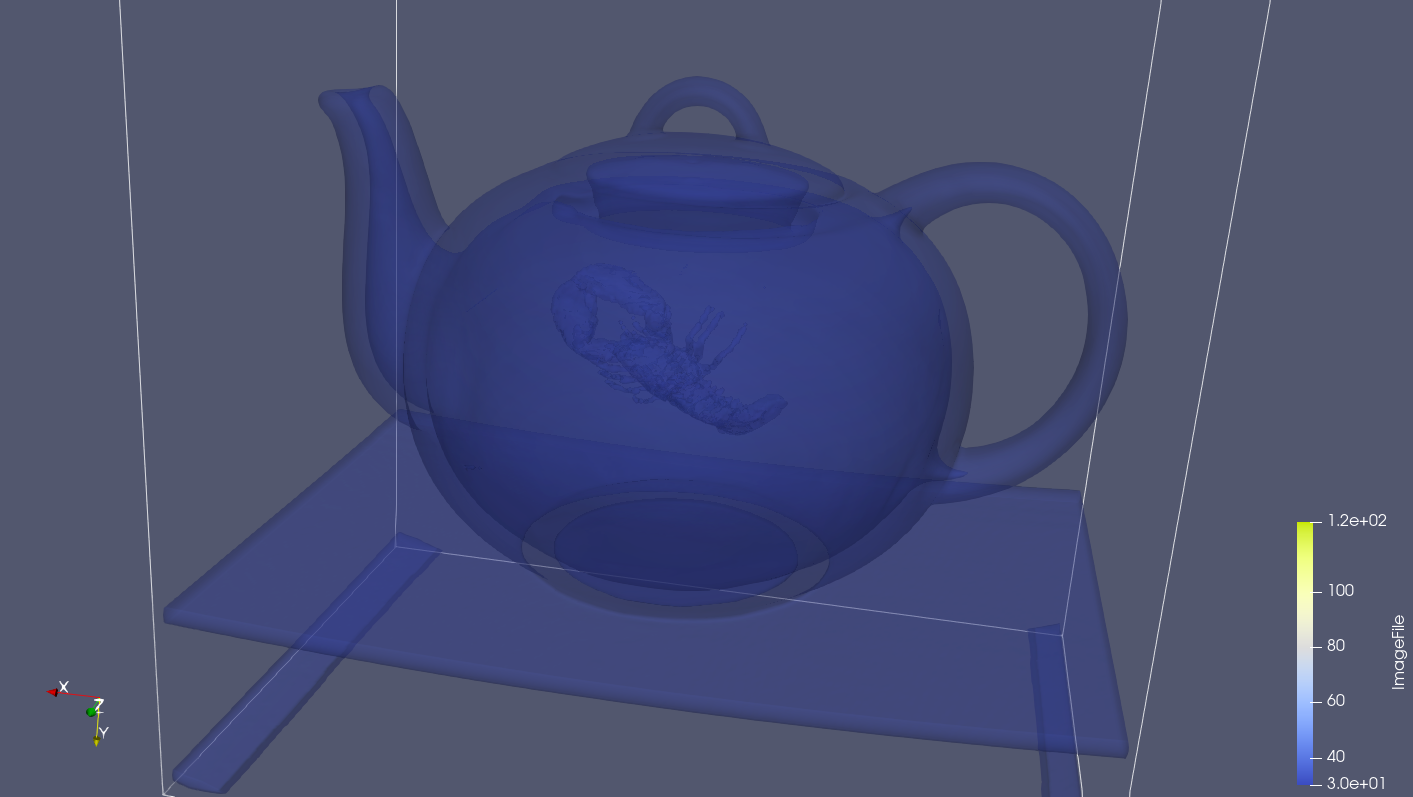
\includegraphics[width=0.75\textwidth]{../img/teapot-contour.png}
        
        \caption{The teapot visualized using contour with values 30 (blue) and 135 (yellow) along with an opacity value of 0.4 to see the lobster inside.}
        \label{fig:contour}
    \end{figure}

    \section{Conclusions}
    The characteristics of the Boston teapot dataset can be successfully visualized in Paraview using both the \textit{IsoVolume} and \textit{Contour} filters, with them giving very similar results with slightly different tweaking possibilites. The conclusions drawn from this was that Paraview is easy to get up and running to make simple visualizations. 

    What was also concluded however was that the \textit{IsoVolume} and \textit{Contour} filters didn't provide much tweaking abilities. With both the filters a feature to distinctly highlight the lobster and teapot differently was looked for, this was sort of possible with the \textit{Contour} filter but not in a completely satisfactory way. A way to make only the blue layer transparent while keeping the yellow fully solid was explored but not achieved. This is either a limitation in Paraview or wasn't found through exploring and googling, but would be a nice way to visualize a dataset like this. 

    \newpage
    % \printbibliography

\end{document}